\documentclass[10pt]{book}
\usepackage{setspace}
\usepackage[utf8]{inputenc}
\usepackage[T1]{fontenc}
\usepackage{caption}
\usepackage[font={scriptsize}]{caption}
\usepackage{caption}
\usepackage{lmodern}
\usepackage{geometry}
\geometry{a4paper, left=20mm, right=20mm, top=20mm, bottom=20mm}
\usepackage{graphicx}
\usepackage{float}
\usepackage{setspace}
\setlength{\parindent}{0pt}
\setlength{\parskip}{1em}
\setlength{\headheight}{14pt}
\usepackage{tabularx}
\usepackage{amsmath, amssymb}
\usepackage{siunitx}
\usepackage{circuitikz}
\usepackage{fancyhdr}
\usepackage{pgfplots}
\pgfplotsset{compat=1.18}
\pagestyle{fancy}
\fancyhf{}
\fancyhead[C]{The Workbench}
\fancyfoot[C]{\thepage}
\renewcommand{\headrulewidth}{0pt}
\renewcommand{\footrulewidth}{0pt}
\newcommand{\defn}{\par\noindent\textbf{Definition: }}
\title{My Notebook}
\date{\vfill\today}
\author{Lucas Helal}
\begin{document}
\maketitle
\thispagestyle{fancy}
\newpage
\chapter{Mathematical and Physics Background}

\section{Universal Topics}

\subsection{Scientific Notation and International Standards}

\subsubsection{SI Notation}

The \emph{International System of Units (SI)} is the modern form of the metric system and is the most widely used system of measurement. 
The SI system uses a set of base units and derived units to define the quantities used in scientific and engineering calculations. 
The base units are defined by the \emph{International System of Units (SI)} as follows: 

\emph{Universal Standards}

\begin{itemize} 
  \item Meter (m) - length, a fundamental dimension
  \item Kilogram (kg) - mass, a fundamental dimension
  \item Second (s) - time, a fundamental dimension
  \item Ampere (A) - electric current, rate of flow of electric charge (Coulombs per second), a derivative function with respect to time
  \item Kelvin (K) - temperature, a fundamental dimension
  \item Mole (mol) - amount of substance, a fundamental dimension
  \item Candela (cd) - luminous intensity, power per unit solid angle, a derived dimension (power divided by angle)
\end{itemize}

\emph{Derived Units}

\begin{itemize}
  \item Newton (N) - force, mass times acceleration ($kg \cdot m/s^2$)
  \item Joule (J) - energy, force times distance ($N \cdot m = kg \cdot m^2/s^2$)
  \item Watt (W) - power, energy per unit time ($J/s = kg \cdot m^2/s^3$)
  \item Pascal (Pa) - pressure, force per unit area ($N/m^2 = kg/(m \cdot s^2)$)
  \item Ohm ($\Omega$) - electric resistance, voltage per unit current ($V/A = kg \cdot m^2/(s^3 \cdot A^2)$)
  \item Volt (V) - electric potential, work per unit charge ($J/C = kg \cdot m^2/(s^3 \cdot A)$)
  \item Farad (F) - capacitance, charge per unit voltage ($C/V = s^4 \cdot A^2/(kg \cdot m^2)$)
  \item Henry (H) - inductance, magnetic flux per unit current ($Wb/A = kg \cdot m^2/(s^2 \cdot A^2)$)
  \item Siemens (S) - electrical conductance, reciprocal of resistance ($1/\Omega = s^3 \cdot A^2/(kg \cdot m^2)$)
  \item Weber (Wb) - magnetic flux, magnetic field times area ($T \cdot m^2 = kg \cdot m^2/(s^2 \cdot A)$)
  \item Tesla (T) - magnetic field, magnetic flux per unit area ($Wb/m^2 = kg/(s^2 \cdot A)$)
  \item Coulomb (C) - electric charge, current times time ($A \cdot s$)
  \item Lumen (lm) - luminous flux, light power ($cd \cdot sr$)
  \item Lux (lx) - illuminance, light power per unit area ($lm/m^2 = cd \cdot sr/m^2$)
\end{itemize}

\emph{Prefixes}

\begin{table}[ht]
  \centering
  \begin{tabular}{|c|c|}
  \hline
  \textbf{Prefix} & \textbf{Factor} \\
  \hline
  Yotta (Y) & $10^{24}$ \\
  Zetta (Z) & $10^{21}$ \\
  Exa (E) & $10^{18}$ \\
  Peta (P) & $10^{15}$ \\
  Tera (T) & $10^{12}$ \\
  Giga (G) & $10^{9}$ \\
  Mega (M) & $10^{6}$ \\
  Kilo (k) & $10^{3}$ \\
  Hecto (h) & $10^{2}$ \\
  Deca (da) & $10^{1}$ \\
  Deci (d) & $10^{-1}$ \\
  Centi (c) & $10^{-2}$ \\
  Milli (m) & $10^{-3}$ \\
  \hline
  \end{tabular}
  \caption{SI Prefixes}
  \label{table:si_prefixes}
  \end{table}

\emph{Relevant Mathematical, Physical and Chemical Constants}

\begin{table}[ht]
  \centering
  \begin{tabular}{|c|c|c|}
  \hline
  \textbf{Constant} & \textbf{Value} & \textbf{Unit/Field} \\
  \hline
  \multicolumn{3}{|c|}{\textbf{Mathematical Constants}} \\
  \hline
  Pi ($\pi$) & 3.14159265358979323846 & Geometry \\
  Euler's number (e) & $\approx$ 2.71828 & Calculus \\
  Golden ratio ($\phi$) & $\approx$ 1.61803 & Algebra \\
  Imaginary unit (i) & $\sqrt{-1}$ & Complex numbers \\
  Euler–Mascheroni constant ($\gamma$) & $\approx$ 0.57721 & Number theory \\
  \hline
  \multicolumn{3}{|c|}{\textbf{Physical Constants}} \\
  \hline
  Speed of light in vacuum ($c$) & $\approx 3.00 \times 10^{8}$ & m/s \\
  Planck's constant ($h$) & $\approx 6.63 \times 10^{-34}$ & J s \\
  Reduced Planck's constant ($\hbar$) & $\approx 1.05 \times 10^{-34}$ & J s \\
  Gravitational constant ($G$) & $\approx 6.67 \times 10^{-11}$ & m$^3$ kg$^{-1}$ s$^{-2}$ \\
  Electron charge ($e$) & $\approx 1.60 \times 10^{-19}$ & C \\
  \hline
  \multicolumn{3}{|c|}{\textbf{Chemical Constants}} \\
  \hline
  Avogadro's number ($N_A$) & $\approx 6.02 \times 10^{23}$ & mol$^{-1}$ \\
  Boltzmann's constant ($k_B$) & $\approx 1.38 \times 10^{-23}$ & J/K \\
  Gas constant ($R$) & $\approx 8.31$ & J/(mol K) \\
  Faraday's constant ($F$) & $\approx 96485$ & C/mol \\
  Stefan-Boltzmann constant ($\sigma$) & $\approx 5.67 \times 10^{-8}$ & W/(m$^2$ K$^4$) \\
  \hline
  \end{tabular}
  \caption{Important Mathematical, Physical and Chemical Constants}
  \label{table:constants}
  \end{table}

\newpage
\subsubsection{Standards Reference}

\paragraph{ISO (International Organization for Standardization):}
\begin{itemize}
    \item ISO 9001: Quality Management Systems
    \item ISO 14001: Environmental Management Systems
    \item ISO 27001: Information Security Management
    \item ISO 31000: Risk Management
    \item ISO 80000-2: Mathematical signs and symbols to be used in the natural sciences and technology
    \item ISO 8601: Representation of dates and times
    \item ISO 3166-1: Country codes
    \item ISO/IEC 5218: Codes for the representation of human sexes
    \item ISO/IEC 15418: GS1 Application Identifiers and ASC MH10 Data Identifiers and maintenance
    \item ISO/IEC 15459: Unique identifiers
    \item ISO/IEC 15459-4: Individual transport units
    \item ISO/IEC 15459-6: Groupings
    \item ISO/IEC 19762-1: Harmonized vocabulary
    \item ISO/IEC 19762-4: RFID for Item Management
    \item ISO/IEC 20248: Symbology data carrier identification
\end{itemize}

\paragraph{DIN (Deutsches Institut für Normung):}
\begin{itemize}
    \item DIN 476: Paper sizes (now replaced by ISO 216)
    \item DIN 72552: Terminal designations in automotive electrical systems
    \item DIN 82079: Preparation of instructions for use
    \item DIN 931: Hexagon head bolts with shank
    \item DIN 933: Hexagon head bolts with thread up to head
    \item DIN 912: Hexagon socket head cap screws
    \item DIN 7985: Cross recessed pan head screws
\end{itemize}

\paragraph{IEC (International Electrotechnical Commission):}
\begin{itemize}
    \item IEC 60038: Standard voltages
    \item IEC 60529: Degrees of protection provided by enclosures (IP Code)
    \item IEC 60950: Safety of information technology equipment
    \item IEC 61000: Electromagnetic compatibility (EMC)
\end{itemize}

\paragraph{IEEE (Institute of Electrical and Electronics Engineers):}
\begin{itemize}
    \item IEEE 802.3: Ethernet
    \item IEEE 802.11: Wireless Networking (Wi-Fi)
    \item IEEE 754: Floating-Point Arithmetic
    \item IEEE 1588: Precision Time Protocol
    \item IEEE 802.15.1: Bluetooth
    \item IEEE 802.16: Broadband Wireless Access (WiMAX)
\end{itemize}

\paragraph{NBR/NR (Norma Brasileira Regulamentadora):}
\begin{itemize}
    \item NR 10: Safety in Electrical Installations and Services
    \item NR 12: Safety in Work with Machines and Equipment
    \item NBR 5410: Electrical Installations in Low Voltage
    \item NR 35: Work at Height
    \item NR 17: Ergonomics
    \item NR 18: Working Conditions and Environment in the Construction Industry
    \item NBR 10126: Technical Drawing
    \item NBR 14565: Procedures for data communication network within commercial buildings
    \item NBR IEC 60079-11: Electrical apparatus for explosive gas atmospheres
    \item NBR 8403: Application of lines in technical drawings
\end{itemize}

\newpage
\subsubsection{Error Tolerances}
\begin{table}[ht]
  \centering
  \begin{tabular}{|c|c|c|}
  \hline
  \textbf{Tolerance} & \textbf{Field} & \textbf{Impact} \\
  \hline
  $\pm$ 0.1 mm & Hand Tools Manufacturing & Impacts tool precision and fit \\
  $\pm$ 5\% & Power Generation Voltage & Impacts system performance and safety \\
  $\pm$ 1\% & Power Transmission Voltage & Impacts system performance and safety \\
  $\pm$ 0.5\% & Power Distribution Voltage & Impacts system performance and safety \\
  $\pm$ 1\% & Electronics (Resistance, Capacitance, Inductance) & Impacts circuit performance \\
  $\pm$ 0.5\% & Electronics (Voltage) & Impacts circuit performance \\
  $\pm$ 0.1\% & Electronics (Grounding) & Impacts system safety and performance \\
  $\pm$ 1°C & Electronics (Temperature) & Impacts component lifespan and performance \\
  $\pm$ 0.5 ULP & Computational Algebra (Floating Point) & Impacts accuracy of calculations \\
  \hline
  \end{tabular}
  \caption{Acceptable Error Tolerances and Their Impacts}
  \label{table:tolerances}
  \end{table}

  \newpage
  \subsubsection{Error Tolerances for Multimeters and Ammeters}
  
  \paragraph{Residential Circuits:}
  \begin{itemize}
      \item AC Voltage: $\pm$ 1.5\% - Impacts safety and device performance
      \item DC Voltage: $\pm$ 0.5\% - Impacts safety and device performance
      \item AC Current: $\pm$ 2.5\% - Impacts safety and device performance
      \item DC Current: $\pm$ 2.0\% - Impacts safety and device performance
      \item Resistance: $\pm$ 0.5\% - Impacts safety and device performance
      \item Continuity: $\pm$ 0.1\% - Impacts safety and device performance
      \item Capacitance: $\pm$ 1.0\% - Impacts safety and device performance
  \end{itemize}
  
  \paragraph{Industrial Circuits:}
  \begin{itemize}
      \item AC Voltage: $\pm$ 1.0\% - Impacts safety, device performance, and costs
      \item DC Voltage: $\pm$ 0.5\% - Impacts safety, device performance, and costs
      \item AC Current: $\pm$ 1.5\% - Impacts safety, device performance, and costs
      \item DC Current: $\pm$ 1.0\% - Impacts safety, device performance, and costs
      \item Resistance: $\pm$ 0.5\% - Impacts safety, device performance, and costs
      \item Continuity: $\pm$ 0.1\% - Impacts safety, device performance, and costs
      \item Capacitance: $\pm$ 1.0\% - Impacts safety, device performance, and costs
  \end{itemize}

\newpage
\chapter{Electrical Circuits I}
\section{Resistors}

\subsection{Resistor Notation - Algebraic Definition}

\defn{Resistor}{A resistor is a two-terminal passive electrical component that implements electrical resistance as a circuit element.}

\begin{displaymath}
    \begin{circuitikz}
        \draw (0,0) to[R, l=$R$] (2,0);
    \end{circuitikz}
\end{displaymath}

\defn{Algebraic Definition}{The algebraic definition of a resistor is given by Ohm's Law, which states that the current through a conductor between two points is directly proportional to the voltage across the two points.}

\begin{equation}
    D: v \longrightarrow i \quad \text{where} \quad v = i \cdot R
    V = i \cdot R
\end{equation}

\begin{itemize}
  \item{Resistance as a function of voltage and current}
  \item{Unit \[\frac{V}{A} = \Omega\]}
\end{itemize}

\newpage

\subsection{Resistor Notation - Geometric Definition}
\defn{Geometric Definition}{The geometric definition of a resistor is given by the resistor's physical properties, such as its length, cross-sectional area, and resistivity.}

% resistor diagram
\begin{displaymath}
    \begin{circuitikz}
        \draw (0,0) to[R, l=$R$, a=$\rho$] (2,0);
    \end{circuitikz}
\end{displaymath}

\begin{equation}
  R = \rho \cdot \frac{l}{A}
\end{equation}
where: 
\begin{itemize}
  \item{$R$ is the resistance of the resistor}
  \item{$\rho$ is the resistivity of the material}
  \item{$l$ is the length of the resistor}
  \item{$A$ is the cross-sectional area of the resistor}
\end{itemize}

\newpage
\subsubsection{Geometrical Interpretation of Resistance as Relationship between Voltage and Current}.

Let's consider the following diagram, which represents a resistor with a voltage source connected to it. The voltage source creates an electric field within the resistor, which causes the free electrons to move in the direction of the electric field. This movement of electrons creates a current flow through the resistor.
% graph of resistance and its derivative
\begin{displaymath}
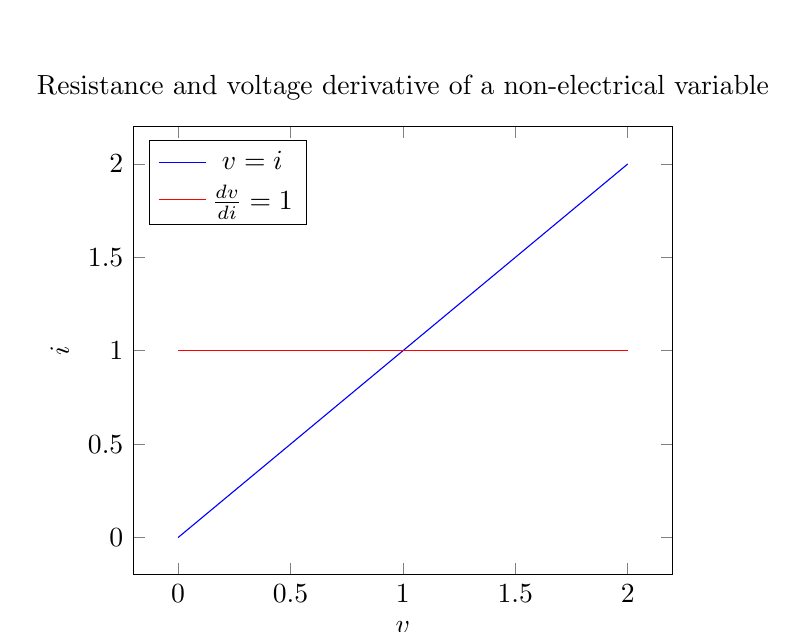
\begin{tikzpicture}
\begin{axis}[
    title={Resistance and voltage derivative of a non-electrical variable},
    xlabel={$v$},
    ylabel={$i$},
    domain=0:2,
    samples=100,
    legend pos=north west
]
\addplot [blue] {x}; % v = i (linear function)
\addlegendentry{$v = i$}

\addplot [red] {1}; % derivative of v = i (constant function)
\addlegendentry{$\frac{dv}{di} = 1$}
\end{axis}
\end{tikzpicture}
\end{displaymath}

\newpage

\section{Circuit Analysis}

\subsection{Kirchhoff's Laws}

\defn{Kirchhoff's Laws}{Kirchhoff's Laws are two fundamental laws that govern the behavior of electrical circuits.}

\emph{There is two things to consider: devices and topology restrictions.}

\begin{itemize}
  \item{Kirchhoff's Current Law (KCL)}
  \item{Kirchhoff's Voltage Law (KVL)}
  \item{Devices: resistors, capacitors, inductors, etc.}
\end{itemize}

\subsubsection{Kirchhoff's Current Law - KCL}

\defn{Kirchhoff's Current Law}{Kirchhoff's Current Law states that the sum of currents entering a node is equal to the sum of currents leaving a node.}

\begin{equation}
  \sum_{i=1}^{n} i_{\text{in}} = \sum_{i=1}^{n} i_{\text{out}}
\end{equation}


\begin{quote}

  The circuit diagrams above illustrate \emph{Kirchhoff's Current Law}(KCL), 
which states that the algebraic sum of currents entering a node (or a junction) equals zero. 
This principle is a consequence of the conservation of electric charge. 

In the first diagram, we see positive charges $(+)$ flowing into a node. Each arrow represents a current path, 
and the label $i_{\text{in}}^-$ indicates that these are incoming currents. In the second diagram, we see negative charges $(-)$ flowing out of a node, 
which represent electrons moving out of the node, creating a current. 

The arrows again indicate the direction of the current flow, and the label $i_{\text{out}}^-$ indicates that these are outgoing currents. According to KCL, 
the sum of the incoming currents should equal the sum of the outgoing currents at a node, which is visually represented in these diagrams.

\end{quote}

The graph below illustrates the concept of Kirchhoff's Current Law, showing the algebraic sum of currents entering a node equal to zero in the passive convention.

\begin{figure}[ht]
  \centering
  \begin{minipage}{.5\textwidth}
    \centering
    \begin{circuitikz}
      \draw (0,0) node[circ] {} -- (2,0) to[short, i=$i_{\text{in}}^-$] (1,0);
      \draw (0,0) -- (-2,0) to[short, i=$i_{\text{in}}^-$] (-1,0);
      \draw (0,0) -- (0,2) to[short, i=$i_{\text{in}}^-$] (0,1);
      \draw (0,0) -- (0,-2) to[short, i=$i_{\text{in}}^-$] (0,-1);
    \end{circuitikz}
    \caption{{Positive charges $(+)$ flowing into the node}}    
  \end{minipage}%
  \begin{minipage}{.5\textwidth}
    \centering
    \begin{circuitikz}
      \draw (0,0) node[circ] {} -- (1,0) to[short, i=$i_{\text{out}}^-$] (2,0);
      \draw (0,0) -- (-1,0) to[short, i=$i_{\text{out}}^-$] (-2,0);
      \draw (0,0) -- (0,1) to[short, i=$i_{\text{out}}^-$] (0,2);
      \draw (0,0) -- (0,-1) to[short, i=$i_{\text{out}}^-$] (0,-2);
    \end{circuitikz}
    \caption{{Negative charges $(-)$ flowing out of the node}}
  \end{minipage}
\end{figure}

\newpage

\subsubsection{Kirchhoff's Voltage Law - KVL}

\defn{Kirchhoff's Voltage Law}{Kirchhoff's Voltage Law states that the sum of voltages around a closed loop is equal to zero.}

\emph{At any closed loop, the sum of the voltage sources is equal to the sum of the voltage drops.}

\begin{equation}
  \sum_{i=1}^{n} v_{\text{in}} = \sum_{i=1}^{n} v_{\text{out}}
\end{equation}

\begin{quote}
The circuit diagram above represents a node with negative charges flowing out. This is a visualization of 
Kirchhoff's Current Law, which states that the algebraic sum of currents entering a node (or a junction) equals zero. 
In this case, the negative charges represent electrons moving out of the node, which creates a current. \\

The arrows indicate the direction of the current flow. Each arrow represents a current path, and the label \boldmath{$i_{\text{out}}^-$} 
indicates that these are outgoing currents. This diagram is a useful tool for understanding the behavior of electrical circuits, 
particularly the principle of conservation of electric charge, which is the basis of \emph{Kirchhoff's Current Law.}

\end{quote}

\emph{Sum of voltages around a closed loop is equal to zero independent of the direction of the loop.}
\begin{figure}[ht]
  \centering
  \begin{minipage}{.5\textwidth}
    \centering
    \begin{align}
      V_g &= V_1 + V_2 + V_3 \nonumber \\
      &= i_g \cdot R_1 + i_g \cdot R_2 + i_g \cdot R_3 \nonumber \\
      &= i_g \cdot (R_1 + R_2 + R_3) \nonumber \\
      &= i_g \cdot R_{\text{eq}}
  \end{align}
    \caption{{Circuit from $+$ to $-$}}
  \end{minipage}%
  \begin{minipage}{.5\textwidth}
    \centering
    \begin{align}
      V_g &= - V_1 - V_2 - V_3 \nonumber \\
      &\therefore \  R^{+}_{eq} \equiv R^{-}_{eq} \nonumber \\
  \end{align}
    \caption{{Circuit from $-$ to $+$}}
  \end{minipage}
\end{figure}

% example 1 here

\newpage
\subsubsection{{Example I. Kirchhoff's Laws in a Series Circuit with Resistors}}

Consider a simple series circuit with a DC power source and two resistors, as shown below, \textbf{assuming the passive convention}:

\begin{figure}[ht]
  \centering
  \begin{circuitikz}[american voltages]
    \draw (0,0) to[V, l=$V_g$, i=$i_g$] (0,2)
          to[R, l=$R_1$, v=$V_1$] (2,2)
          to[R, l=$R_2$, v=$V_2$] (4,2)
          -- (4,0) -- (0,0);
  \end{circuitikz}
  \caption{Series circuit with a DC power source and two resistors}
\end{figure}

According to Kirchhoff's Voltage Law (KVL), the sum of the voltages around any closed loop in the circuit is equal to zero. For this circuit, the equation is:

\begin{equation}
V_g = V_1 + V_2
\end{equation}

According to Ohm's law, the voltage across a resistor is equal to the current through the resistor times the resistance of the resistor. So we can write:

\begin{align}
V_1 &= i_g \cdot R_1 \\
V_2 &= i_g \cdot R_2
\end{align}

Substituting these equations into the KVL equation, we get:

\begin{equation}
V_g = i_g \cdot R_1 + i_g \cdot R_2 = i_g \cdot (R_1 + R_2)
\end{equation}

This equation tells us that the voltage of the power source is equal to the current through the circuit times the total resistance of the circuit.

According to Kirchhoff's Current Law (KCL), the sum of the currents entering a node (or a junction) equals the sum of the currents leaving the node. For this circuit, the equation is:

\begin{equation}
i_g = i_1 = i_2
\end{equation}

This equation tells us that the current through the power source is equal to the current through each resistor, which is a characteristic of series circuits.

It's important to note that the direction of the loop does not affect the application of KVL. Whether we move in the direction of the current (from $+$ to $-$) or against it (from $-$ to $+$), the sum of the voltages around the loop is still zero. This is true even in the presence of a power source or a load, where the power is negative or positive, respectively.


\newpage
\subsubsection{Example II. Proof that the direction of the loop does not affect the application of KVL}

Consider a simple series circuit with a DC power source and two resistors, as shown below, \textbf{assuming the passive convention}:

\begin{figure}[ht]
  \centering
  \begin{circuitikz}[american voltages]
    \draw (0,0) to[V, l=$V_g$, i=$i_g$] (0,2)
          to[R, l=$R_1$, v=$V_1$] (2,2)
          to[R, l=$R_2$, v=$V_2$] (4,2)
          -- (4,0) -- (0,0);
  \end{circuitikz}
  \caption{Series circuit with a DC power source and two resistors}
\end{figure}

Given the values:

\begin{itemize}
\item Voltage of the power source, $V_g = 12V$
\item Resistance of the first resistor, $R_1 = 2\Omega$
\item Resistance of the second resistor, $R_2 = 3\Omega$
\item Current through the circuit, $i_g = 2A$
\end{itemize}

We can calculate the voltage across each resistor using \textbf{Ohm's law}, $V = i \cdot R$:

\begin{align}
V_1 &= i_g \cdot R_1 = 2A \cdot 2\Omega = 4V \\
V_2 &= i_g \cdot R_2 = 2A \cdot 3\Omega = 6V
\end{align}

Now we can apply \textbf{KVL} in the direction of the current (from $+$ to $-$):

\begin{equation}
V_g - V_1 - V_2 = 0
\end{equation}

Substituting the given values:

\begin{equation}
12V - 4V - 6V = 2V \neq 0
\end{equation}

\textbf{This is not consistent with KVL}. The issue here is that the current $i_g$ is not correct. The current through the circuit should be equal to the voltage of the power source divided by the total resistance of the circuit, according to Ohm's law. So, the correct current is:

\begin{equation}
i_g = \frac{V_g}{R_1 + R_2} = \frac{12V}{2\Omega + 3\Omega} = 2.4A
\end{equation}

Substituting this current into the voltages across the resistors:

\begin{align}
V_1 &= i_g \cdot R_1 = 2.4A \cdot 2\Omega = 4.8V \\
V_2 &= i_g \cdot R_2 = 2.4A \cdot 3\Omega = 7.2V
\end{align}

Substituting these voltages into the KVL equation:

\begin{equation}
12V - 4.8V - 7.2V = 0V
\end{equation}

\textbf{Now, the sum of the voltages around the loop is equal to zero, which is consistent with KVL}. So, the direction of the loop does not affect the application of KVL, as long as we follow the passive sign convention and use the correct current.


\end{document}